\documentclass[border=10pt]{standalone}
\usepackage{tikz}
\usepackage{amsmath}
\usepackage{amssymb}
\usetikzlibrary{positioning, arrows.meta, shapes, calc}

\begin{document}
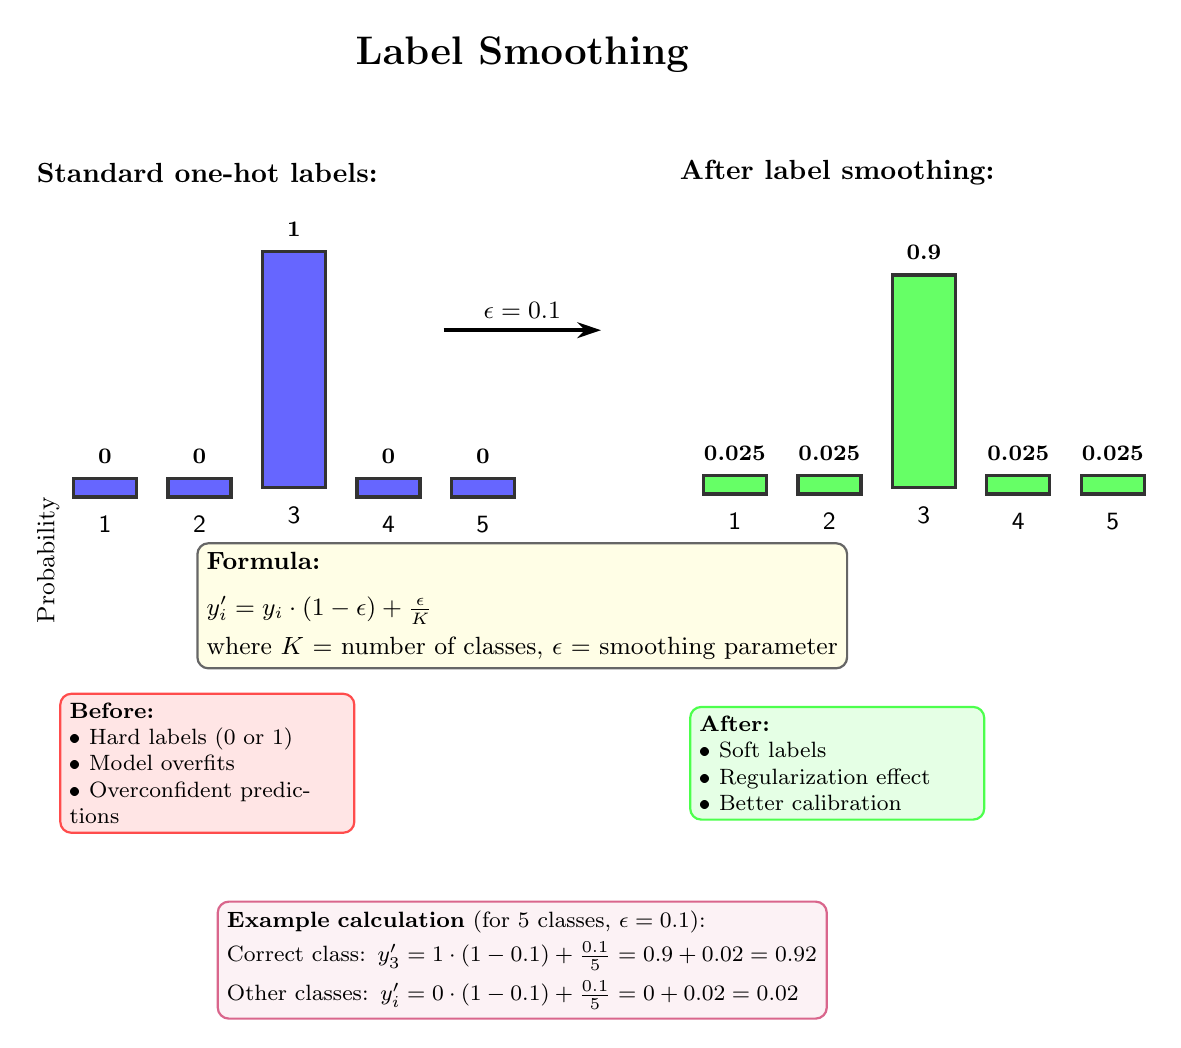
\begin{tikzpicture}[
    font=\sffamily,
    bar/.style={rectangle, minimum height=0.5cm, minimum width=0.8cm, draw=black!80, very thick},
    label/.style={font=\small\sffamily}
]

% Title
\node[font=\Large\bfseries] at (0, 5.5) {Label Smoothing};

% Original One-Hot Labels
\node[font=\bfseries] at (-4, 4) {Standard one-hot labels:};
\foreach \i/\val in {1/0, 2/0, 3/1, 4/0, 5/0} {
    \pgfmathsetmacro{\height}{\val * 3}
    \node[bar, fill=blue!60, minimum height=\height cm] (orig\i) at (-6.5 + \i*1.2, \height/2) {};
    \node[below=0.1cm of orig\i, label] {\i};
    \node[above=0.05cm of orig\i, font=\footnotesize\bfseries] {\val};
}
\node[left=0.3cm of orig1, rotate=90, font=\small] {Probability};

% Arrow
\draw[-{Stealth[length=3mm, width=2mm]}, ultra thick] (-1, 2) -- (1, 2) 
    node[midway, above, font=\small\bfseries] {$\epsilon = 0.1$};

% Smoothed Labels
\node[font=\bfseries] at (4, 4) {After label smoothing:};
\foreach \i/\val in {1/0.025, 2/0.025, 3/0.9, 4/0.025, 5/0.025} {
    \pgfmathsetmacro{\height}{\val * 3}
    \node[bar, fill=green!60, minimum height=\height cm] (smooth\i) at (1.5 + \i*1.2, \height/2) {};
    \node[below=0.1cm of smooth\i, label] {\i};
    \node[above=0.05cm of smooth\i, font=\footnotesize\bfseries] {\val};
}

% Formula box
\node[draw=black!60, fill=yellow!10, rounded corners, thick, align=left, font=\small] at (0, -1.5) {
    \textbf{Formula:} \\[0.2cm]
    $y'_i = y_i \cdot (1 - \epsilon) + \frac{\epsilon}{K}$ \\[0.1cm]
    where $K$ = number of classes, $\epsilon$ = smoothing parameter
};

% Annotations
\node[draw=red!70, fill=red!10, rounded corners, thick, align=left, font=\footnotesize, text width=3.5cm] 
    at (-4, -3.5) {
    \textbf{Before:} \\
    • Hard labels (0 or 1) \\
    • Model overfits \\
    • Overconfident predictions
};

\node[draw=green!70, fill=green!10, rounded corners, thick, align=left, font=\footnotesize, text width=3.5cm] 
    at (4, -3.5) {
    \textbf{After:} \\
    • Soft labels \\
    • Regularization effect \\
    • Better calibration
};

% Example calculation
\node[draw=purple!60, fill=purple!5, rounded corners, thick, align=left, font=\footnotesize, text width=7.5cm] 
    at (0, -6) {
    \textbf{Example calculation} (for 5 classes, $\epsilon = 0.1$): \\[0.1cm]
    Correct class: $y'_3 = 1 \cdot (1 - 0.1) + \frac{0.1}{5} = 0.9 + 0.02 = 0.92$ \\[0.1cm]
    Other classes: $y'_i = 0 \cdot (1 - 0.1) + \frac{0.1}{5} = 0 + 0.02 = 0.02$
};

\end{tikzpicture}
\end{document}